\documentclass[]{beamer}

\mode<presentation>{


%%%% ТЕМЫ %%%%
% \usetheme{Berlin} %++main++
% \usetheme{Boadilla} %+
% \usetheme{CambridgeUS} %-
% \usetheme{Madrid} %+
\usetheme{Montpellier} % свобода в названиях, секциях и подсекциях
% \usetheme{Pittsburgh} %минимализм
% \usetheme{Szeged} %классический, без авторов, с нижней строкой


%%%% ЦВЕТА %%%%
\usecolortheme{beaver} %+осень
% \usecolortheme{crane} %+осень?
% \usecolortheme{dolphin}
% \usecolortheme{dove} %+беленький
% \usecolortheme{seagull} %+business
% \usecolortheme{seahorse} %+winter
% \usecolortheme{whale} %+winter
% \usecolortheme{spruce} %+spring


%%%% ДРУГИЕ НАСТРОЙКИ %%%%
%\setbeamertemplate{footline} % To remove the footer line in all slides uncomment this line
%\setbeamertemplate{footline}[frame number] % To replace the footer line in all slides with a simple slide count uncomment this line
\setbeamertemplate{navigation symbols}{} % Чтобы удалить символы навигации со дна всех скользких скользких
\setbeamercovered{transparent} % Раскрывает серые анимации (полезные для дизайна, но могут быть прокомментированы при передаче окончательного документа)
% Использовать шрифт вспышки везде
\usefonttheme{serif}
}

\usepackage[T2A]{fontenc}
\usepackage[utf8]{inputenc}
\usepackage[english]{babel}
\usepackage{hyperref}     % ТАК_НУЖНО
\hypersetup{unicode=true} % ТАК_НУЖНО
\usepackage{amsmath}
\usepackage{amssymb,textcomp, esvect,esint}
\usepackage{amsfonts}
\usepackage{amsthm}
\usepackage{graphicx}
\usepackage{indentfirst}
\usepackage{xcolor}
% \usepackage{enumitem} %--- ломал нумерацию!?

\usepackage{graphicx}
\usepackage{booktabs}
\usepackage{caption}
\usepackage{listings}
\usepackage{tikz}
\usepackage{xcolor}



\usepackage{media9}
\usepackage{animate}
\usepackage{threeparttable}
\usepackage{pifont}


\usepackage{import}
\usepackage{xifthen}
\usepackage{pdfpages}
\usepackage{transparent}

% \usepackage{natbib}

\usepackage[skip=1pt]{caption}

\usepackage{ifthen}
\definecolor{darkgreen}{RGB}{10,90,10}
% базовая подстройка
\renewcommand{\d}{\, d}
\renewcommand{\leq}{\leqslant}
\renewcommand{\geq}{\geqslant}


% авторские команды
\newcommand{\vc}[1]{\mbox{\boldmath $#1$}}
\newcommand{\smallvc}[1]{\scalebox{0.65}{\mbox{\boldmath $#1$}}}
\newcommand{\T}{^{\text{T}}}
\newcommand{\con}{^{\dag}}
\newcommand{\sub}[2]{#1_{\textnormal{#2}}}
\newcommand{\vp}{\vphantom{\dfrac{1}{2}}}

% операторы (просто прямой текст)
\renewcommand{\Im}{\mathop{\mathrm{Im}}\nolimits}
\renewcommand{\Re}{\mathop{\mathrm{Re}}\nolimits}
% \renewcommand{\P}{\mathop{\mathrm{P}}\nolimits}
% \newcommand{\E}{\mathop{\mathrm{E}}\nolimits}
% \newcommand{\D}{\mathop{\mathrm{D}}\nolimits}
\newcommand{\cov}{\mathop{\mathrm{cov}}\nolimits}
\newcommand{\diag}{\mathop{\mathrm{diag}}\nolimits}
\newcommand{\card}{\mathop{\mathrm{card}}\nolimits}
\newcommand{\grad}{\mathop{\mathrm{grad}}\nolimits}
\renewcommand{\div}{\mathop{\mathrm{div}}\nolimits}
\newcommand{\rot}{\mathop{\mathrm{rot}}\nolimits}
\newcommand{\Ker}{\mathop{\mathrm{ker}}\nolimits}
\newcommand{\spec}{\mathop{\mathrm{spec}}\nolimits}
\newcommand{\sign}{\mathop{\mathrm{sign}}\nolimits}
\newcommand{\tr}{\mathop{\mathrm{tr}}\nolimits}
\newcommand{\rg}{\mathop{\mathrm{rg}}\nolimits}
\newcommand{\const}{\textnormal{const}}


% цветной текст
\newcommand{\red}[1]{\textcolor{red}{#1}}
\newcommand{\green}[1]{\textcolor{urlcolor}{#1}}
\newcommand{\blue}[1]{\textcolor{ublue}{#1}}


% символы
\newcommand{\cmark}{\text{\ding{51}}}
\newcommand{\xmark}{\text{\ding{55}}}


% подгрузка pdf_tex картинок
% \newcommand{\incfig}[1]{%
%     \def\svgwidth{\columnwidth}
%     \import{./figures/}{#1.pdf_tex}
% }


% специфично к квантам
\newcommand{\ket}[1]{\left| #1 \right\rangle}
\newcommand{\bra}[1]{\left\langle #1 \right|}

\newcommand{\dppp}{\frac{d^3 p}{(2 \pi \hbar)^3}}

\newcommand{\na}{$^{22}$Na}
\newcommand{\cs}{$^{137}$Cs}
\newcommand{\co}{$^{60}$Co}
\newcommand{\am}{$^{214}$Am}
\newcommand{\eu}{$^{152}$Eu}
% % % \newif\ifbeamer@tree@showhooks
% \beamer@tree@showhookstrue

% \DeclareOptionBeamer{hooks}[true]{\csname beamer@tree@showhooks#1\endcsname}
% \ProcessOptionsBeamer

% \mode<presentation>
% \defbeamertemplate*{headline}{tree theme}
% {%
%     \begin{beamercolorbox}[wd=\paperwidth,colsep=1.5pt]{upper separation line head}
%     \end{beamercolorbox}
%     \begin{beamercolorbox}[wd=\paperwidth,ht=2.5ex,dp=1.125ex,%
%       leftskip=.3cm,rightskip=.3cm plus1fil]{title in head/foot}
%       \usebeamerfont{title in head/foot}\insertshorttitle
%     \end{beamercolorbox}
%     \begin{beamercolorbox}[wd=\paperwidth,ht=2.5ex,dp=1.125ex,%
%       leftskip=.3cm,rightskip=.3cm plus1fil]{section in head/foot}
%       \usebeamerfont{section in head/foot}%
%       \ifbeamer@tree@showhooks
%         \setbox\beamer@tempbox=\hbox{\insertsectionhead}%
%         \ifdim\wd\beamer@tempbox>1pt%
%           \hskip2pt\raise1.9pt\hbox{\vrule width0.4pt height1.875ex\vrule width 5pt height0.4pt}%
%           \hskip1pt%
%         \fi%
%       \else%  
%         \hskip6pt%
%       \fi%
%       \insertsectionhead
%     \end{beamercolorbox}
%     \begin{beamercolorbox}[wd=\paperwidth,ht=2.5ex,dp=1.125ex,%
%       leftskip=.3cm,rightskip=.3cm plus1fil]{subsection in head/foot}
%       \usebeamerfont{subsection in head/foot}%
%       \ifbeamer@tree@showhooks
%         \setbox\beamer@tempbox=\hbox{\insertsubsectionhead}%
%         \ifdim\wd\beamer@tempbox>1pt%
%           \hskip9.4pt\raise1.9pt\hbox{\vrule width0.4pt height1.875ex\vrule width 5pt height0.4pt}%
%           \hskip1pt%
%         \fi%
%       \else%  
%         \hskip12pt%
%       \fi%
%       \insertsubsectionhead
%     \end{beamercolorbox}
%     \begin{beamercolorbox}[wd=\paperwidth,colsep=1.5pt]{lower separation line head}
%     \end{beamercolorbox}
% }

  
% \mode
% <all>





\newcommand{\progressbar}{% 
	\pgfmathsetmacro{\slidewidth}{\paperwidth}
	\pgfmathsetmacro{\progressstep}{\paperwidth/\inserttotalframenumber}
	\pgfmathsetmacro{\progresspos}{(\insertframenumber - 0.5) * \progressstep}
	\begin{tikzpicture}[scale = 0.035, line width = 1ex]
		\node[inner sep=0pt] (cat) at (\progresspos,0)	{
\includegraphics[width=30pt]{settings/cats/cat_red.pdf}};
		\path[red] (0,0) -- (\slidewidth,0);
	\end{tikzpicture}
}

\makeatletter
\setbeamertemplate{footline}
{
\hfill 
% \progressbar %включить котика
    \leavevmode%
    \hbox{
    \begin{beamercolorbox}[wd=.33\paperwidth,ht=2.25ex,dp=1ex,center]{section in head/foot}
        \insertshortauthor~~\beamer@ifempty{\insertshortinstitute}{}{(\insertshortinstitute)} % раскомментить для авторов
        % \insertshortinstitute % раскомментить для вуза
    \end{beamercolorbox}%
    \begin{beamercolorbox}[wd=.33\paperwidth,ht=2.25ex,dp=1ex,center]{section in head/foot}
        % \insertshortdate{}
        \insertshorttitle
    \end{beamercolorbox}%
    \begin{beamercolorbox}[wd=.33\paperwidth,ht=2.25ex,dp=1ex,right]{section in head/foot}%
        \insertframenumber/\inserttotalframenumber \hspace{1mm}
    \end{beamercolorbox}
    }%
}

%
% \usebeamerfont{author in head/foot}\insertshortauthor~~\beamer@ifempty{\insertshortinstitute}{}{(\insertshortinstitute)} % раскомментить для авторов
% \usebeamerfont{author in head/foot}\beamer@ifempty{\insertshortinstitute}{}{\insertshortinstitute}
% \usebeamerfont{title in head/foot}\insertshorttitle
%   % \usebeamerfont{date in head/foot}\insertshortdate{}\hspace*{2em}
%   % \insertframenumber{} / \inserttotalframenumber\hspace*{2ex} 
% \insertshortinstitute \insertframenumber/\inserttotalframenumber


%%% Логотип
% \usepackage{tikz}
% \addtobeamertemplate{headline}{}{%
% \begin{tikzpicture}[remember picture,overlay]
% \node at([shift={(5.5,-0.5)}]current page.north) {
\includegraphics[height=.8\headheight]{settings/cat.png}};
% \end{tikzpicture}}



%%% добавить сетку %%%
% \setbeamertemplate{background}{\tikz[overlay, remember picture, help lines]{
%     \foreach \x in {0,...,12} \path (current page.south west) +(\x,0.5) node {\small$\x$};
%     \foreach \y in {0,...,9} \path (current page.south west) +(0.5,\y) node {\small$\y$};
%     \foreach \x in {0,0.5,...,12.5} \draw (current page.south west) ++(\x,0) -- +(0,9.6);
%     \foreach \y in {0,0.5,...,9.5} \draw (current page.south west) ++(0,\y) -- +(12.8,0);
%   }
% }


%%% верхняя полоска с точками %%%
\setbeamertemplate{headline}
{%
  % \begin{beamercolorbox}[colsep=1.5pt]{upper separation line head}
  % \end{beamercolorbox}
  \begin{beamercolorbox}{section in head/foot}
    \vskip0pt\insertnavigation{\paperwidth}\vskip2pt
  \end{beamercolorbox}%
  \begin{beamercolorbox}[colsep=1.5pt]{lower separation line head}
  \end{beamercolorbox}
}
% \setbeamertemplate{headline}{}


%%% добавить маленькие номера слайдов справа снизу %%%
% \addtobeamertemplate{navigation symbols}{}{%
%     \usebeamerfont{footline}%
%     \usebeamercolor[myred]{footline}%
%     \hspace{1em}%
%     \insertframenumber/\inserttotalframenumber
% }




\setbeamertemplate{frametitle}{%
    \nointerlineskip%
    \begin{beamercolorbox}[wd=\paperwidth,ht=2.0ex,dp=0.6ex]{frametitle}
        \hspace*{1ex}\insertframetitle%
    \end{beamercolorbox}%
}
\title[Hydrogen orbitals]{Hydrogen Wave Function}

\author{
Khoruzhii K., Primak E.}
\institute[MIPT]

\begin{document}
\date{21.07.2021}
\maketitle


\frame{
\begin{minipage}{0.35\textwidth}
      Possible applications:
\end{minipage}
\hfill
\begin{minipage}{0.63\textwidth}
    \begin{itemize}
    	\iitem{optical reflectometry;}
    	\iitem{chaos radar;}
        \iitem{random numbers generation;}
        \iitem{signal encryption.}
    \end{itemize}
\end{minipage}
 \frametitle{Title}}

\frame{
% quantum microscope

\xmark \ making many weak measurements of a quantum system

\cmark \  a series of strong measurements on identically prepared systems 

\begin{figure}[h]
    \centering
    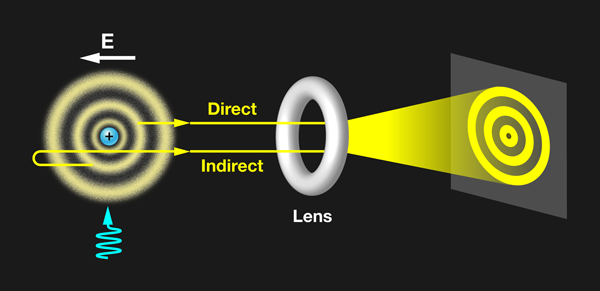
\includegraphics[width=0.75\textwidth]{figures/1.png}
    %\caption{}
    %\label{fig:}
\end{figure}


\cmark applying a dc electric field that defines a quantization axis in hydrogen and aligns the orbitals before measuring them \frametitle{Idea of <<quantum microscope>>}}

\frame{
\begin{minipage}{0.55\textwidth}
    \begin{figure}[h]
    \centering
    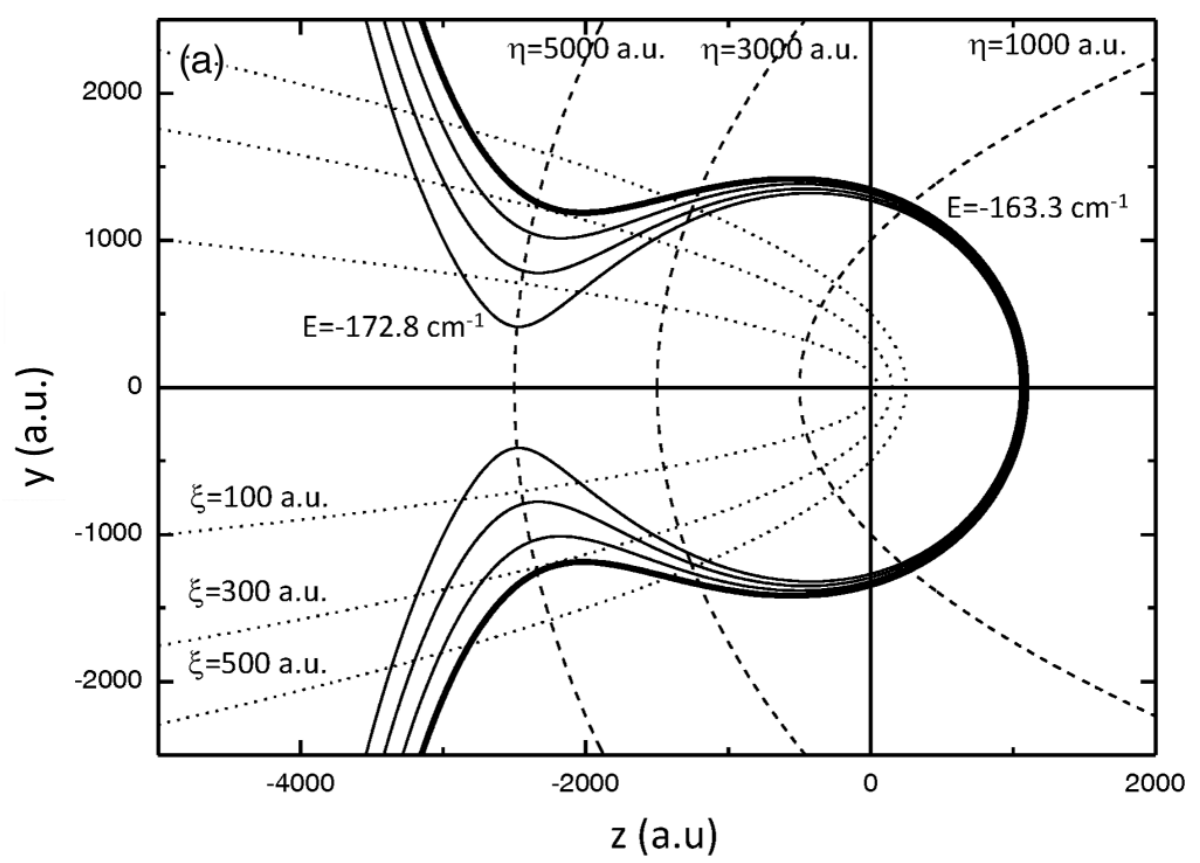
\includegraphics[width=1.1\textwidth]{figures/parabola.png}
    % \caption{}
    %\label{fig:}
\end{figure}
\end{minipage}
\hfill
\begin{minipage}{0.35\textwidth}
    % В статическом электрическом поле волновая функция водорода может быть разделена в смысле параболических координат
    For $z$ --- displacement along the electric field.
    And $r$ --- electron-proton distance.
    \begin{gather*}
    	\eta = r - z \\
    	\xi  = r + z 
    \end{gather*}
\end{minipage}
\begin{equation*}
	\Psi(\xi,\eta,\varphi) = \frac{1}{\sqrt{2 \pi \eta \xi}} \chi_1(\xi) \chi_2(\eta) e^{i m \varphi}
\end{equation*}
 \frametitle{Geometry of the problem}}

\frame{
\begin{figure}[h]
    \centering
    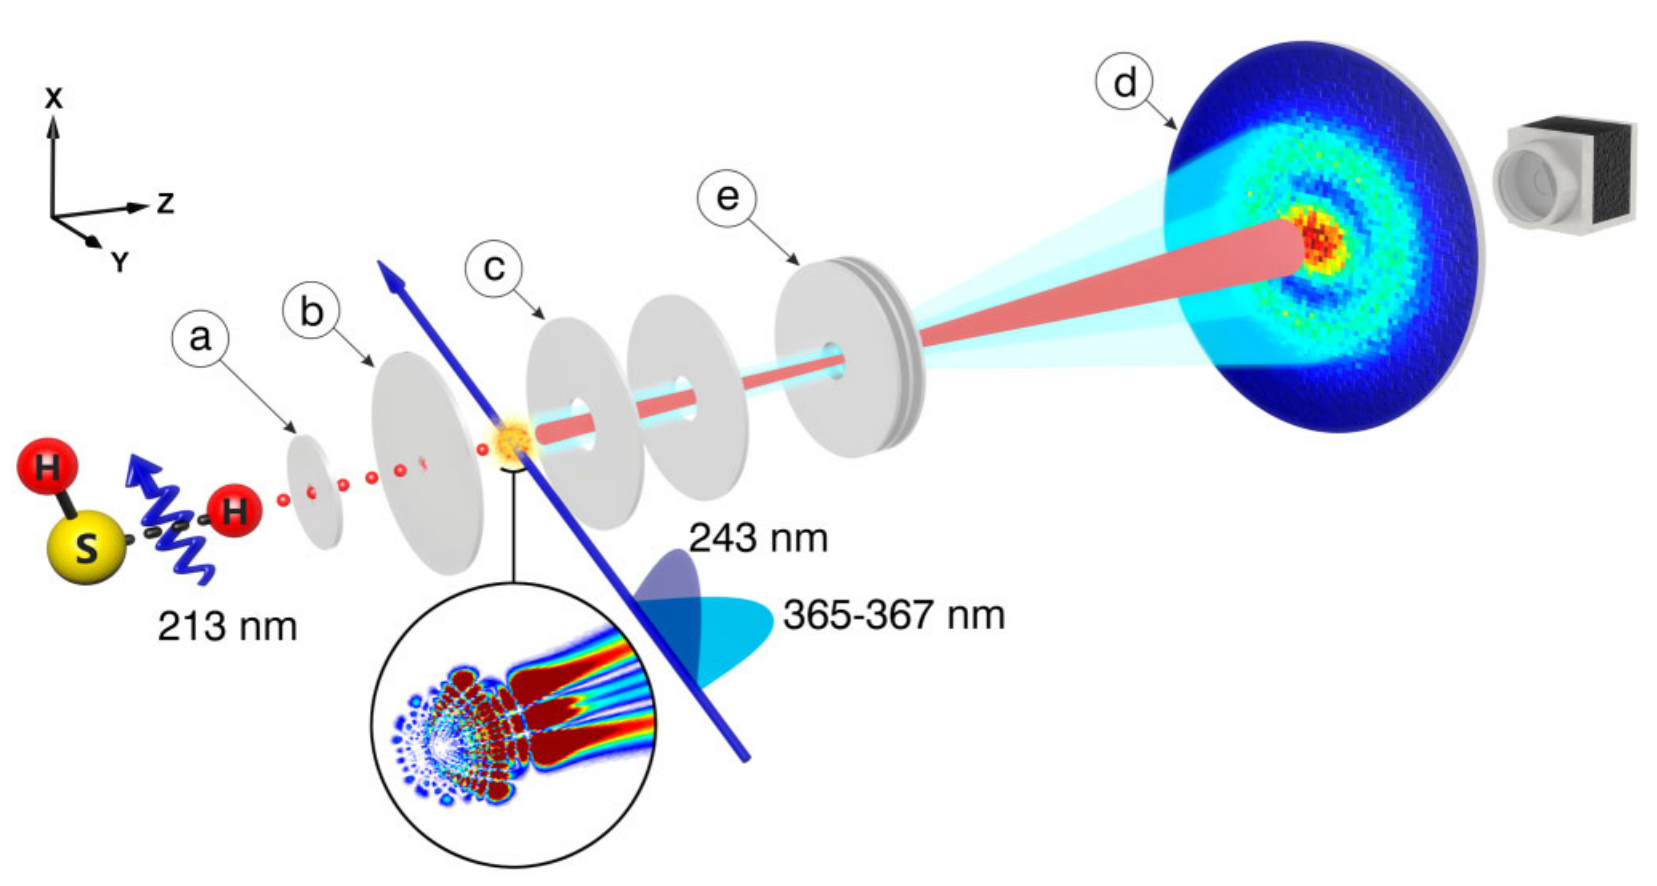
\includegraphics[width=0.75\textwidth]{figures/2.png}
    %\caption{}
    %\label{fig:}
\end{figure}
 \frametitle{Preparation of state}}

\frame{
Experimental observation of the transverse nodal structure of four atomic hydrogen Stark states
\begin{minipage}{0.55\textwidth}
    \begin{figure}[h]
        \centering
        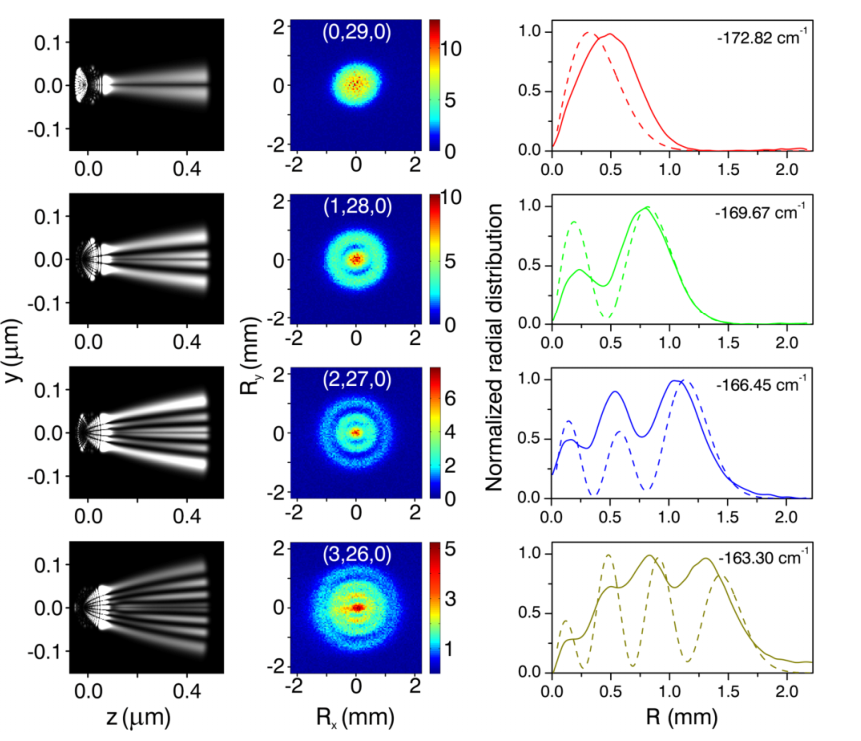
\includegraphics[height=0.95\textwidth]{figures/3.png}
    \end{figure}
\end{minipage}
\hfill
\begin{minipage}{0.35\textwidth}
    % \begin{figure}[h]
    %     \centering
    %     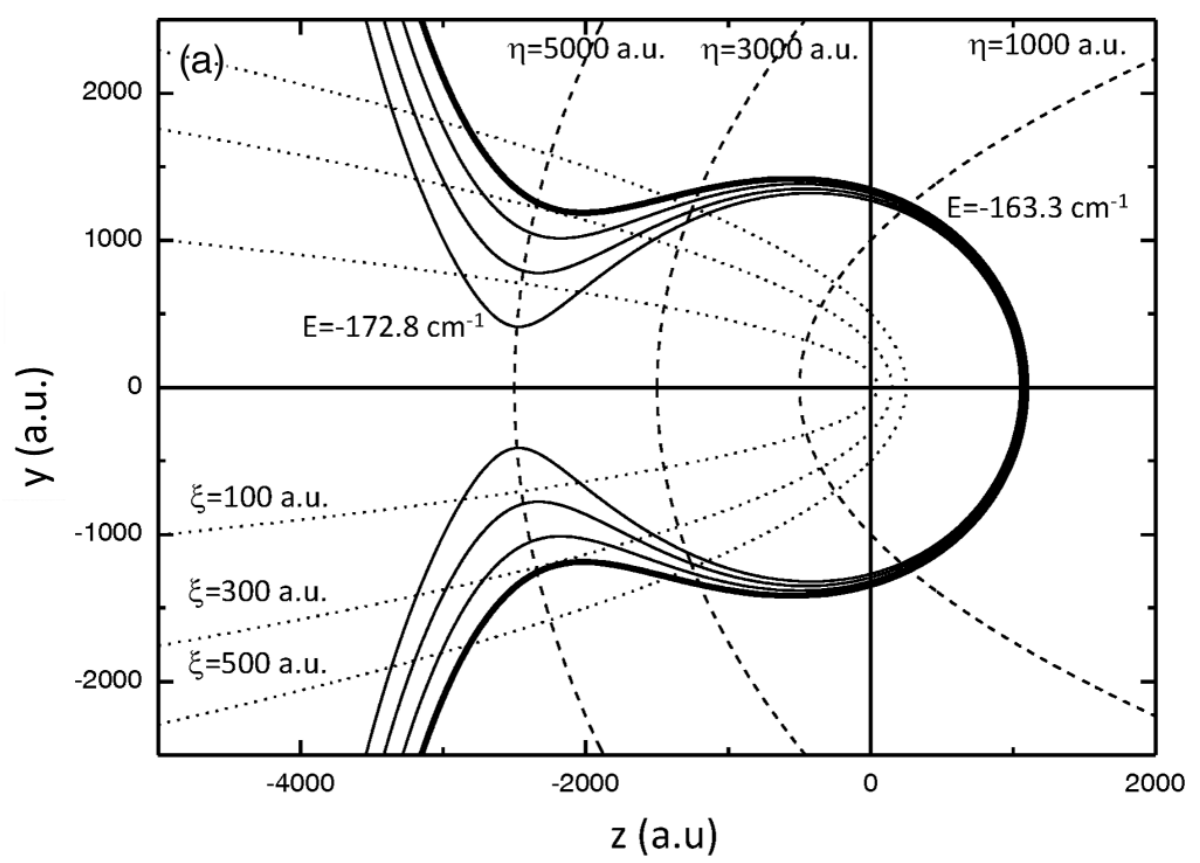
\includegraphics[width=1\textwidth]{figures/parabola.png}
    %     \caption{$n = n_1 + n_2 + |m| + 1$}
    %     %\label{fig:}
    % \end{figure}
         States $(n_1,n_2,m)$ 

        \cmark $m$ --- the magnetic quantum number. 

        \cmark $n_1, n_2$ --- related to the principal quantum number as\\
        $
            n = n_1 + n_2 + |m| + 1
        $
\end{minipage}


 \frametitle{Experimental observation}}

\frame{
Experimental observation of the transverse nodal structure of four atomic hydrogen Stark states
\begin{minipage}{0.55\textwidth}
    \begin{figure}[h]
        \centering
        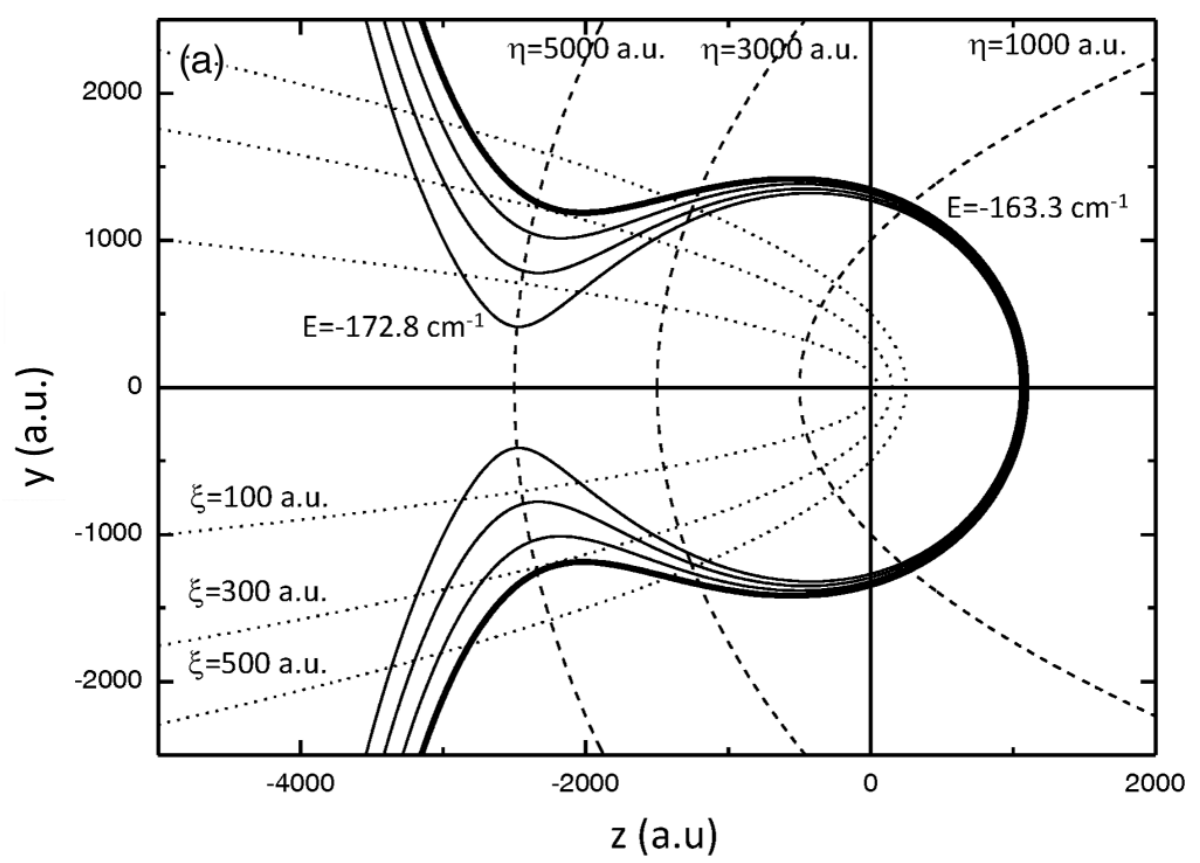
\includegraphics[height=0.8\textwidth]{figures/parabola.png}
    \end{figure}
\end{minipage}
\hfill
\begin{minipage}{0.35\textwidth}
    % \begin{figure}[h]
    %     \centering
    %     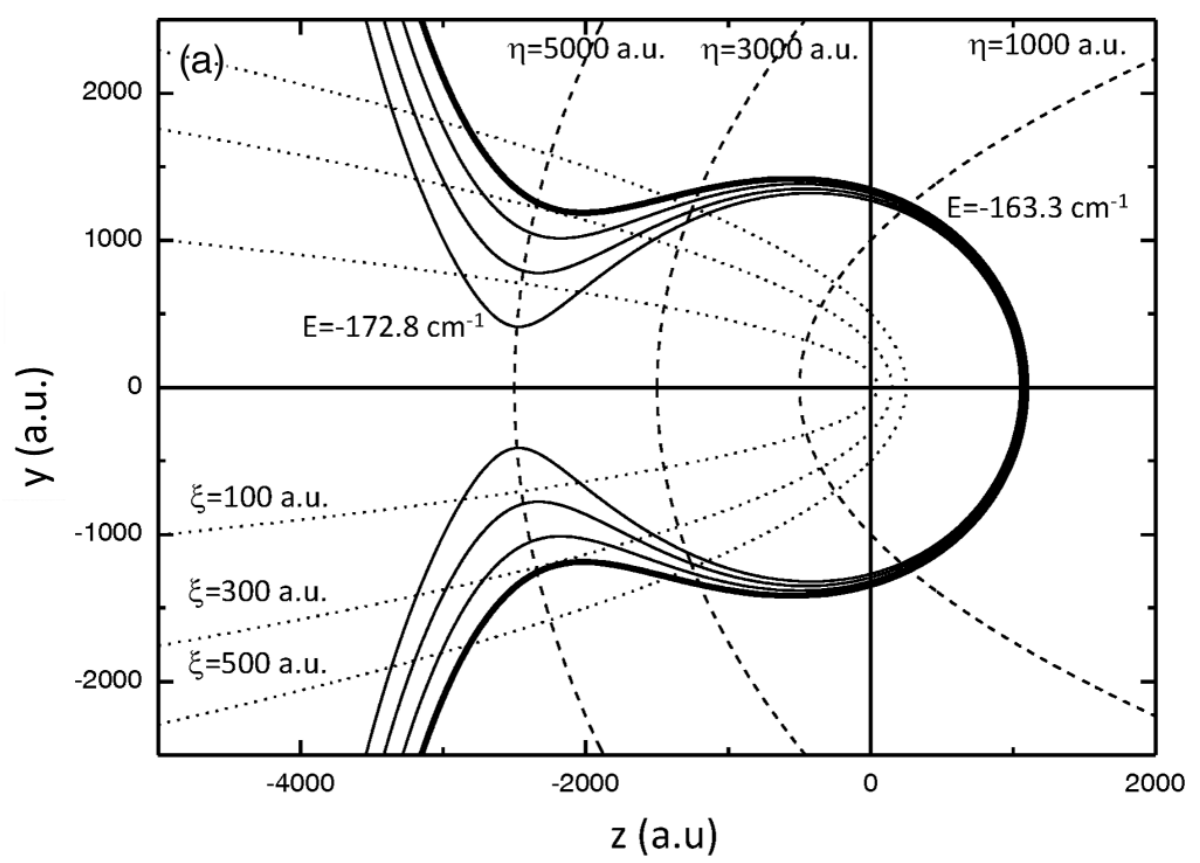
\includegraphics[width=1\textwidth]{figures/parabola.png}
    %     \caption{$n = n_1 + n_2 + |m| + 1$}
    %     %\label{fig:}
    % \end{figure}
         States $(n_1,n_2,m)$ 

        \cmark $m$ --- the magnetic quantum number. 

        \cmark $n_1, n_2$ --- related to the principal quantum number as\\
        $
            n = n_1 + n_2 + |m| + 1
        $
\end{minipage}


 \frametitle{Experimental observation}}

\frame{
Experimental observation of the transverse nodal structure of four atomic hydrogen Stark states
\begin{minipage}{0.55\textwidth}
    \begin{figure}[h]
        \centering
        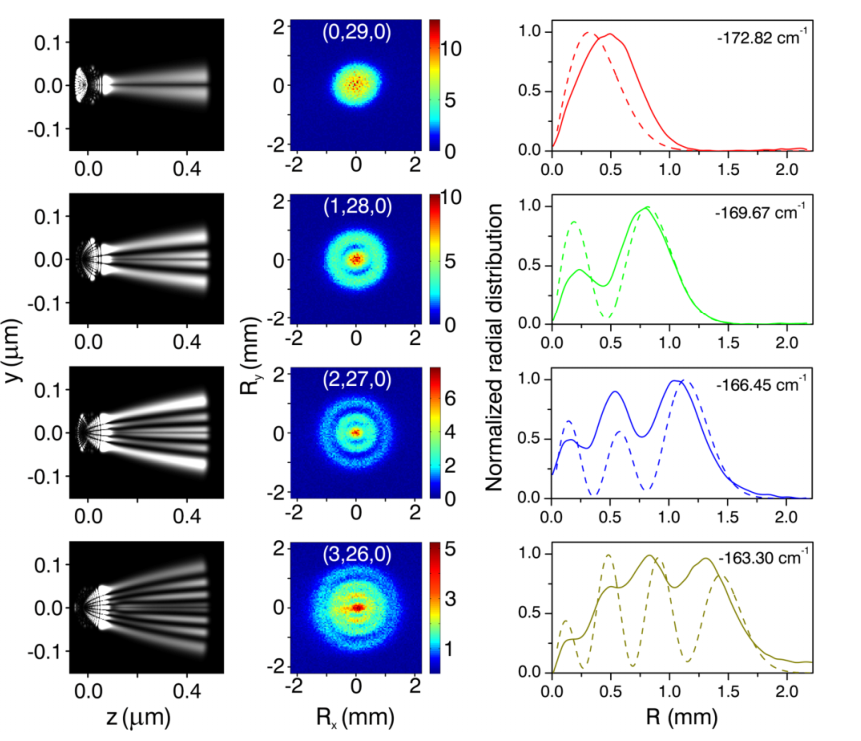
\includegraphics[height=0.95\textwidth]{figures/3.png}
    \end{figure}
\end{minipage}
\hfill
\begin{minipage}{0.35\textwidth}
    % \begin{figure}[h]
    %     \centering
    %     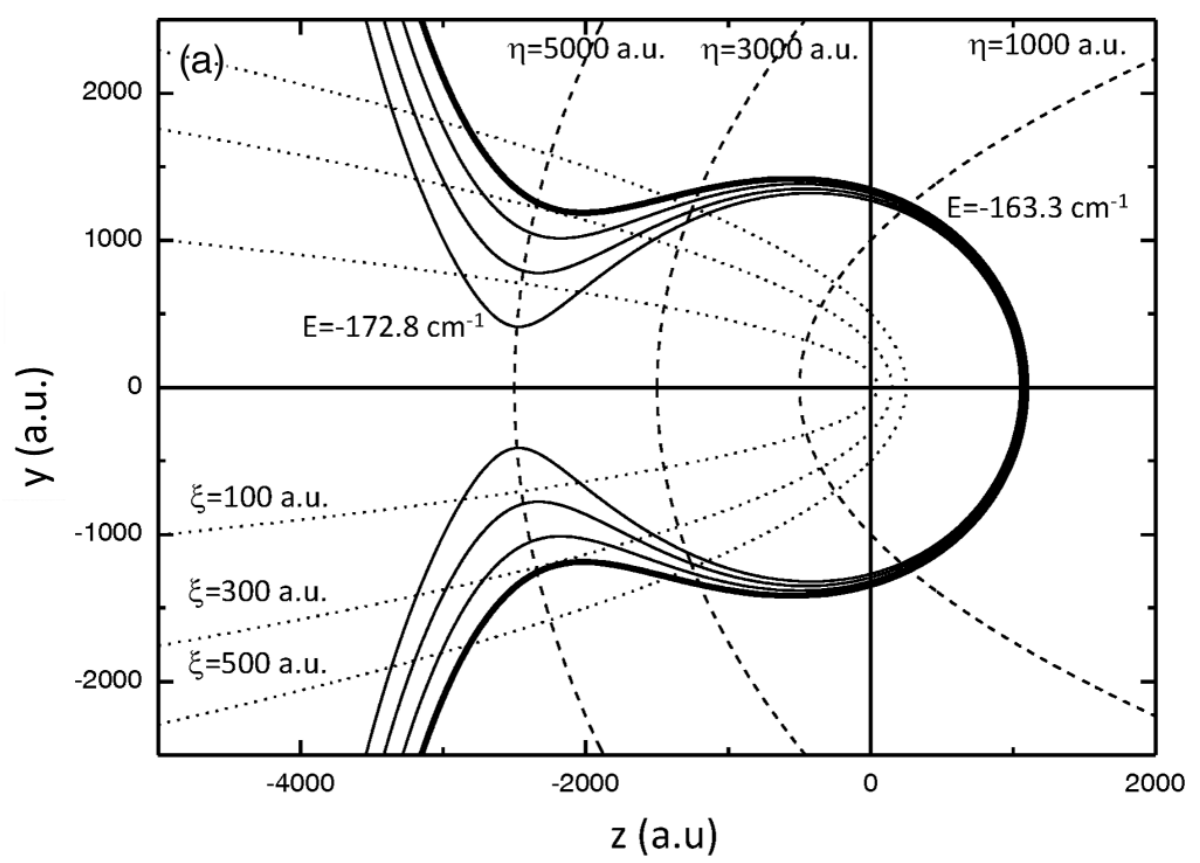
\includegraphics[width=1\textwidth]{figures/parabola.png}
    %     \caption{$n = n_1 + n_2 + |m| + 1$}
    %     %\label{fig:}
    % \end{figure}
        States $(n_1,n_2,m)$ 

        \cmark $m$ --- the magnetic quantum number. 

        \cmark $n_1, n_2$ --- related to the principal quantum number as\\
        $
            n = n_1 + n_2 + |m| + 1
        $
\end{minipage}


 \frametitle{Experimental observation}}

% \frame{
% \input{slides/3_01.tex} \frametitle{Title}}


% \input{slides/1_chaos.tex}

% \input{slides/2_motion_eqs_theory.tex}

% \input{slides/3_feedback_idea.tex}

% \input{slides/2_short_feedback_idea.tex} Женя хочет в своем рассказе вопроса по выбору это раскоментить
% \input{slides/2_short_feedback_idea.tex} можно и раскоментить, но зачем теория, если она и так валяется в конце?

% \input{slides/5_feedback_implementation.tex}
% 
% \input{slides/4_motion_eqs_modeling.tex}

% \input{slides/7_light_braches.tex}

% \input{slides/K1_experiment.tex}

% \input{slides/5_5_feedback_problems.tex}

% \input{slides/6_conclusion.tex}

% \frame[noframenumbering]{
% \input{slides/e_00.tex} \frametitle{Literature}}

% % \input{slides/9_aftermath.tex}


\end{document}



